% -*- compile-command: "pdflatex --enable-write18 max-flow.tex" -*-
\documentclass{tufte-handout}

\usepackage{algo-activity}
%\usepackage{programB}

\title{Algorithms: Max Flow}
\date{}

\begin{document}

\maketitle

\begin{questions}

\item Consider the graph in Model \ref{graph1} and the algorithm below. The algorithm claims to find in a graph $V, E$ the maximum flow $f(e) \forall e in E$ through the graph. On line 3, it arbitrarily chooses an unsaturated path and adds flow to it. What is an ordering of choices that enables this algorithm to successfully find a maximum flow?

\begin{objective}
  Students will derive an efficient algorithm for finding the flow of maximum value in a graph.
\end{objective}

\begin{enumerate}
    \item Initialize $f(e) \leftarrow 0$ for all $e \in E$
    \item repeat
    \item \hspace{1cm} Find an unsaturated path $P$ from $s$ to $t$
    \item \hspace{1cm} $a \leftarrow$ minimum excess capacity $c(e) - f(e)$ among all edges $e \in P$
    \item \hspace{1cm} $f(e) \leftarrow f(e) + a$ for each edge $e \in P$
    \item until no more unsaturated $s \leftarrow t$ paths
\end{enumerate}

\item What is an ordering of choices that prevents this algorithm from finding a maximum flow?

%\begin{algorithm*}[h]
%\caption{{\sc GreedyFlow}} \label{alg:greedy}
%\begin{algorithmic}[1]
%\medskip
%\State Initialize $f(e) \gets 0$ for all $e \in E$
%\Repeat
%\State Find an unsaturated path $P$ from $s$ to $t$
%\State $a \gets$ minimum excess capacity $c(e) - f(e)$ among all edges
%$e \in P$
%\State $f(e) \gets f(e) + a$ for each edge $e \in P$
%\Until{no more unsaturated $s \to t$ paths}
%\end{algorithmic}
%\end{algorithm*}

\begin{model}{Graph}{graph}
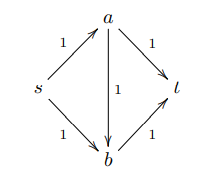
\includegraphics{Flow_POGIL_1.png}
\label{graph1}
\end{model}

\begin{model}{Flow Graphs}{graph_flow_b}
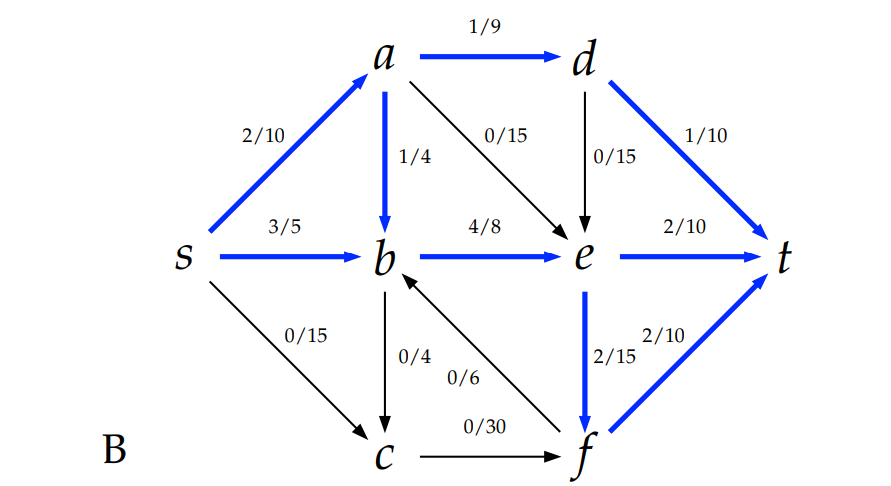
\includegraphics[scale=.68]{Flow_POGIL_2.png}
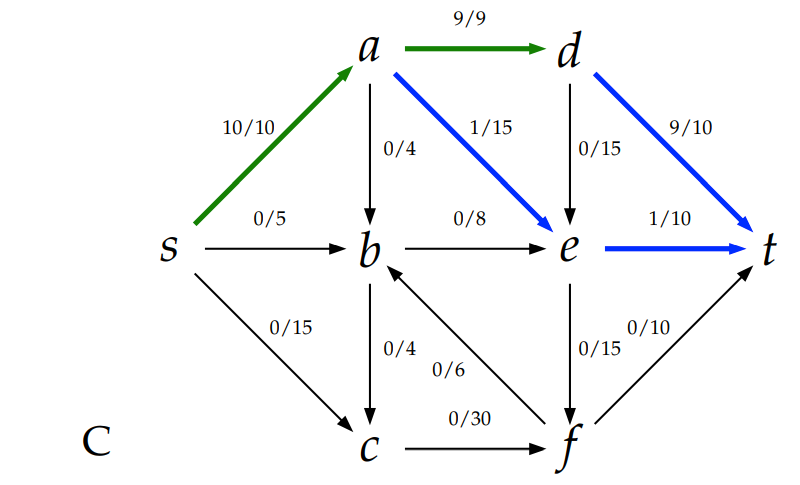
\includegraphics[scale=.68]{Flow_POGIL_3.png}
\label{graph_flow_b}
\end{model}

\begin{defn}
  Given a network $G=(V,E)$ and a flow $f$ on $G$, we define the
  \term{residual graph} $G_{f}$ as $G_{f}=(V,E_f)$, with
  \[ E_f = \{ e \in E \mid c(e) - f(e) > 0 \} \cup \{ e^R \mid e \in
    E, f(e) > 0 \} \] (where $e^R$ denotes the reverse of edge $e$)
  and we define the capacities of edges in $E_f$ by
  \begin{itemize}
  \item $c_{f}(e)=c(e)-f(e)$, and
  \item $c_{f}(e^{R}) = f(e)$.
  \end{itemize}
\end{defn}

\item Based on the given definition of a residual graph, draw a residual graph for each of the flow graphs depicted in Model \ref{graph_flow_b}.

\newpage

\item Consider the algorithm below. 

\begin{enumerate}
    \item Initialize $f(e) \leftarrow 0$ for all $e \in E$
    \item repeat
    \item \hspace{1cm} $\alpha \leftarrow \min\{ c_{f}(e) \,|\, e \in P\}$ \label{line:augmenta}
    \item \hspace{1cm} $f(e) \leftarrow f(e) + \alpha$ for each $e \in P$ such that $e \in E$  \label{line:augmentb}
    \item \hspace{1cm} $f(e) \leftarrow f(e) - \alpha$ for each $e \in P$ such that $e^{R} \in E$  \label{line:augmentc}
    \item until no paths exist from $s$ to $t$ in $G_f$
\end{enumerate}

This algorithm, the Ford-Fulkerson algorithm, uses the  residual graph $G_f$ instead of the original graph to find \term{augmenting paths}. We execute lines~\ref{line:augmenta},~\ref{line:augmentb}
and~\ref{line:augmentc} because we have found an augmenting path
in the residual graph.

Use the Ford-Fulkerson algorithm to find a flow on the graph in Model \ref{original_graph}. Select paths in any order you like. 

\begin{model}{Original Graph}{graph}
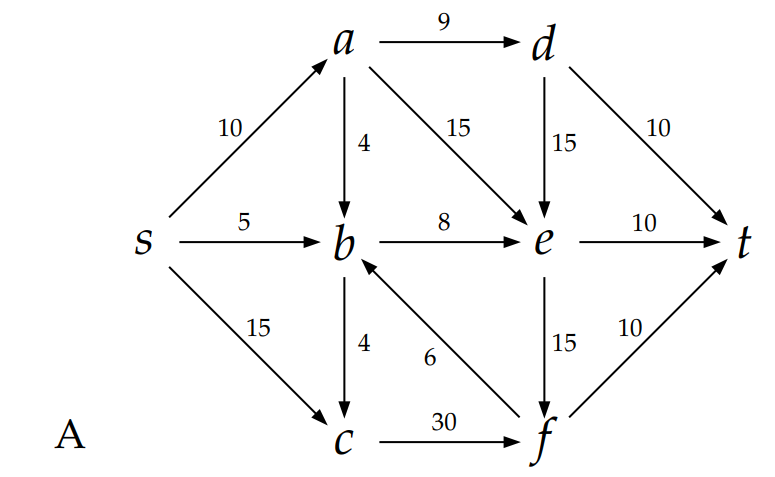
\includegraphics[scale=.68]{Flow_POGIL_4.PNG}
\label{original_graph}
\end{model}

\item Is the flow you computed in the previous question the maximum possible flow? Why or why not?

\end{questions}

\end{document}
